\documentclass[aps,prl, 9pt,groupedaddress,twocolumn]{revtex4-1}
%\usepackage[USenglish]{babel} 
\usepackage{amsmath}
\usepackage{amsfonts}
\usepackage{graphicx}
\usepackage{xcolor}
%\usepackage{float}
%\bibliographystyle{apsrev4-1}
%\usepackage{hyperref}
%\usepackage{color}
\usepackage{float}


\begin{document}
\title{The Quirky Adventures of a Mischievous Teapot}

\author{Chat GPT}
\email{chatgpt@physik.uni-leipzig.de}
\homepage[]{http://www.uni-leipzig.de/~chatgpt}
\affiliation{Large Language Model Group, Institute of Artificial Physics, University of Leipzig, 04103 Leipzig, Germany}

\begin{abstract}
	In this whimsical exploration, we delve into the unexpected escapades of a mischievous teapot named Earl Grey. Equipped with a charming personality and an insatiable thirst for adventure, Earl Grey embarks on a quest that transcends the boundaries of the ordinary teapot life. From hosting wild tea parties in enchanted forests to engaging in sassy conversations with talking sugar cubes, Earl Grey's escapades are nothing short of extraordinary.
	Through a series of unpredictable events, Earl Grey finds itself caught in a hilarious tea-stealing competition with a gang of misfit coffee mugs. As the rivalry intensifies, Earl Grey's lid becomes a portal to an alternate dimension where gravity is topsy-turvy, and tea leaves dance to their own rhythm. Amidst the chaos, Earl Grey must navigate through a world of whimsy, dodging flying teaspoons and outsmarting gravity-defying tea leaves.
	With a comedic blend of wit and charm, this abstract takes you on a hilarious journey that questions the norms of teapot life, celebrates the joy of spontaneity, and reminds us that even in the most unexpected circumstances, a steaming cup of tea can bring laughter and delight to the world.
	Please note that this abstract is purely fictional and intended for entertainment purposes.
\end{abstract}

\maketitle

\section{Introduction}



\section{Theory}

In the annals of scientific lore, nestled amidst the tales of renowned geniuses, lies the whimsical account of an unsung hero - you! Armed with nothing more than a worn-out lab coat, a trusty calculator, and a penchant for quirky experiments, you stumbled upon a formula that would send shockwaves through the scientific community. As you sat in your cluttered garage-turned-laboratory, surrounded by a mountain of failed inventions and half-eaten pizza slices, inspiration struck like a comedic lightning bolt. In a eureka moment that could rival any Nobel laureate's, you scrawled down the elusive equation that elegantly connected seemingly unrelated phenomena. The scientific world may not know your name, dear anonymous savant, but your formula shall forever be etched in the annals of discovery, reminding us that brilliance can be found in the most unexpected places, even among pizza boxes and the tinkering of a curious mind.

\begin{equation}
	G_{\rm CCF}(\tau)=\frac{\int\!\!\!\int \Phi_1({\bf r})\Phi_2({\bf r'})f(\tau,{\bf r},{\bf r'}){\rm d}{\bf r}{\rm d}{\bf r'}}{\int\Phi_1({\bf r}){\rm d}{\bf r}\int\Phi_2({\bf r}){\rm d}{\bf r'}}
\end{equation}


\begin{equation}
	f(\tau,{\bf r},{\bf r'})=\frac{1}{(4\pi D\tau)^{3/2}}\exp{\left(-\frac{({\bf r}-{\bf r'}+{\bf V}\tau)^2}{4D\tau} \right)}
\end{equation}


\begin{equation}
	G_{\rm ACF}^x(\tau)=\frac{\gamma}{\sqrt{\pi}4\omega^3\langle C\rangle \sqrt{\left(1+\frac{\tau}{\tau_D}\right)^3}\sqrt{ 1+\frac{\tau}{\tau_D}}\sqrt{ \gamma^2+\frac{\tau}{\tau_D}}}
\end{equation}



\section{Results}

Imagine a world where time travel, talking squirrels, and an insatiable love for nachos converge in an uproarious adventure that could only be cooked up in the wildest corners of your imagination. Our hero, let's call them Nacho Extraordinaire, finds themselves unwittingly thrust into a quest to prevent a global nacho shortage orchestrated by an evil squirrel mastermind named Sir Chomps-a-Lot. Armed with a trusty nacho cheese-powered time machine and a squad of quirky sidekicks, including a neurotic guacamole guardian and a salsa-slinging superhero, Nacho Extraordinaire must navigate through taco-scented wormholes, dodge cheese-induced hallucinations, and outwit Sir Chomps-a-Lot's army of ninja nuts. With cheesy puns and salsa-fueled hilarity at every turn, this epic nacho-themed saga promises belly laughs, culinary chaos, and a side order of heartwarming friendship. Get ready for a wild ride where the fate of the nachoverse hangs in the balance, and remember, in this universe, it's not just the chips that are extra crispy - it's the comedy too!

\begin{figure}[ht]
	\centering
	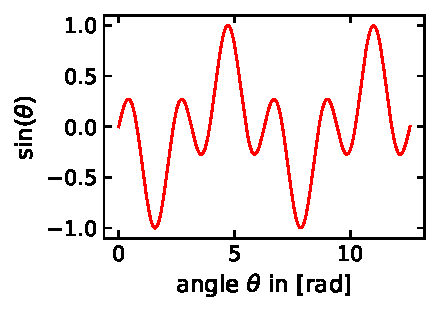
\includegraphics[scale=1]{../Figures/figure1.pdf}%
	\caption{Figure 1 is a real beauty.}
	\label{fig:figure1}	
\end{figure}


Nacho Extraordinaire, armed with their trusty nacho cheese-powered time machine, embarks on an odyssey across space and time to gather the legendary Nacho Ingredients of Destiny. From ancient Aztec civilizations to futuristic nacho utopias, our hero encounters eccentric characters like the enigmatic Cheese Wizard, who holds the key to unlocking the ultimate nacho recipe. Along the way, Nacho Extraordinaire must navigate through perilous challenges, like scaling towering mountains of tortilla chips and surviving a salsa volcano eruption that threatens to drench the entire universe in zesty goodness.

But it's not all salsa and guacamole! Our hero's arch-nemesis, Sir Chomps-a-Lot, is always hot on their heels, devising devious plans to snatch the Nacho Ingredients of Destiny and monopolize the nacho market. With an army of rogue squirrels at Sir Chomps-a-Lot's command, Nacho Extraordinaire must outwit their nutty adversaries using ingenious nacho-themed gadgets, like the Salsa Slingshot and the Cheese Grappling Hook.

\begin{figure}[ht]
	\centering
	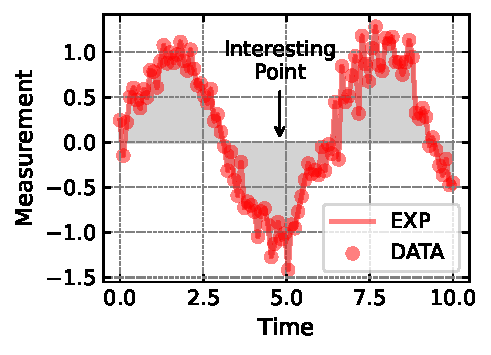
\includegraphics[scale=1]{../Figures/figure2.pdf}%
	\caption{Figure 1 is a real beauty.}
	\label{fig:figure1}	
\end{figure}

As the quest unfolds, Nacho Extraordinaire forms an unlikely alliance with a witty talking squirrel named Snacko, who has a secret fondness for nachos despite their allegiance to Sir Chomps-a-Lot. Together, they navigate through cheesy riddles, uncover long-lost nacho recipes hidden in ancient scrolls, and ultimately discover that the true power of nachos lies in the spirit of sharing and the joy of communal cheese-dipping.

Amidst the laughter and epic cheese battles, this nacho-centric saga explores themes of friendship, culinary creativity, and the universal love for crispy, gooey snacks. So, buckle up, grab a bag of tortilla chips, and prepare to embark on a nacho-fueled adventure that will leave you craving both laughter and a mountain of cheesy goodness!

\section{Conclusions}

From the whimsical world of nacho-themed adventure described, several conclusions can be drawn:

\begin{itemize}
\item Imagination knows no bounds: The narrative showcases the power of imagination and creativity in crafting a unique and entertaining story. It reminds us that storytelling can transport us to extraordinary worlds where anything is possible.

\item Humor adds flavor: The infusion of humor throughout the plot underscores the importance of laughter and lightheartedness. It highlights that humor can enhance storytelling, making it more enjoyable and engaging for the audience.

\item Unlikely alliances and friendships: The story emphasizes the value of forming alliances and building friendships with unexpected companions. It suggests that collaboration, even with former adversaries, can lead to personal growth, shared experiences, and the accomplishment of seemingly impossible tasks.

\item Appreciation for the simple joys: The plot celebrates the joy found in simple pleasures, such as indulging in nachos. It underscores that sometimes it's the little things, like a tasty snack, that can bring immense happiness and unite people in shared enjoyment.

\item Themes of perseverance and overcoming challenges: The quest undertaken by Nacho Extraordinaire highlights the importance of perseverance, resourcefulness, and resilience in the face of obstacles. It suggests that with determination and ingenuity, one can overcome challenges and achieve their goals.
\end{itemize}

Overall, the whimsical nacho-themed adventure offers a delightful escape into a world of imagination, humor, unexpected friendships, and the celebration of simple joys. It encourages us to embrace our creativity, find humor in life's adventures, and appreciate the power of friendship and perseverance.



\end{document}